\section{Probing extra galactic sources}
%In this section one will look at different observables and methods of probing extra galactic sources as potential candidates for the origin of the UHECRs and/or neutrinos. The goal is to constrain our list of candidates by applying known effects and theoretical models to observed data. In brief one will be discussing, The hillas criterion, the anisotropy of the UHECRs and neutrinoes, "the emissivity of our sources in UHECRs and neutrinos", and a comprehensive time scale analysis of the sources.

In this section one will outline some different methods and observables used to probe extra galactic sources as potential candidates for the origin of the UHECRs and/or neutrinos. The goal is to constrain our list of candidates by applying known effects and theoretical models to observed data, and to discuss the implications of these constraints. In brief, one will be discussing the energy budget of our sources, the anisotropy of the UHECRs and neutrinos, and a comprehensive time-scale analysis of the sources. In order to do so several key pieces of information is required, which will be discussed in the following sections.


\subsection{Density and anisotropy}

In order to estimate 

\subsection{SED broad band analysis}
\subsubsection{X-ray luminosity}
\subsubsection{Radio luminosity}
\subsubsection{Photon fields around AGN}


\subsection{Magnetic field constraints}

\subsubsection{Equipartition}
\subsubsection{Self synchrotron absorption}


The theory of synchrotron self absorption is a tool used previously for estimating magnetic field strength in spherically symmetric synchrotron sources. Synchrotron radiation is the product of charged particles traveling in a magnetic field. The radiation is emitted when the particles are accelerated which happens when an electron is spiraling in an uniform magnetic field. The light is usually highly polarized and is dependent on the electron energy and the magnetic field strength. Moving further along, synchrotron self absorption is the process where the synchrotron radiation is absorbed by the same electrons that produced it, and the effect of this is that any given volume of emitting plasma that radiate synchrotron radiation will have a frequency below which the radiation is absorbed. This frequency is called the turnover frequency, and one aims to show how one can estimate the magnetic field strength in the emitting plasma based on this information. The concept was first introduced by \cite{1983ApJ...264..296M}, but this section relies heaviliy on \cite{Hirotani_2005} for the derivation. 

Before we begin the derivation it is fitting to understand the spectrum of synchrotron radiation from a plasma. The spectrum is characterized by the peak frequency, also called the turnover frequency $\nu_m$, the peak flux density $S_m$, and naturally the spectral index $\alpha$. One referse the reader to image \ref{fig:synchrotron_spectrum} for a simple view of the synchrotron speaktrum in question. 

\begin{figure}
    \centering
    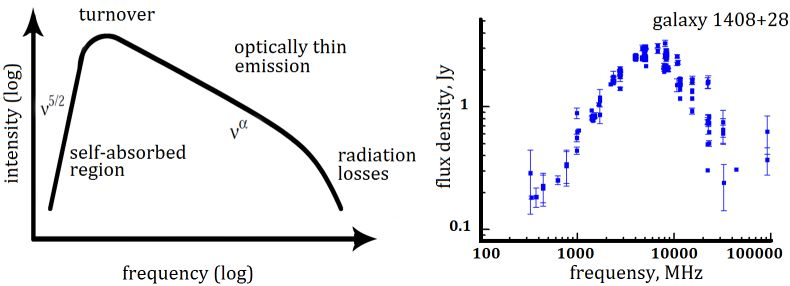
\includegraphics[width=0.5\textwidth]{C:/Users/henri/OneDrive/Documents/NTNU/Semester 10/Masteroppgave/Plots/SYN_spec.jpg}
    \caption{The synchrotron spectrum of a Giga hertz peaked galaxy. Later on one will realise that GHP galaxies and CSO occupy that same niche. Image taken from  Group of Active Galactic Nuclei investigation at https://www.sao.ru/hq/giag/gps-en.html }
    \label{fig:synchrotron_spectrum}
\end{figure}

In order to estimate the magnetic field strenght we must assume that it is uniform and that the electron density is also uniform. From here the transfer equation for synchrotron radiation gives in \cite{Hirotani_2005} gthe specific intensity as 

\begin{equation}
    I_\nu = A(\alpha) \nu^{*\frac{5}{2}}[1-exp(-\alpha_\nu^*x_0^* )] 
\end{equation}
where 

\begin{equation}
    A(\alpha) = \frac{3}{2}^{-\alpha}\frac{e}{c}\frac{a(\alpha)}{C(\alpha)}\left(\frac{e}{2\pi m_e c}\right)^{-3/2}B^{-1/2}
\end{equation}

and $x_0^*$ give the thickness of the emitting plasma along the observers line of sight. The coefficients $a(\alpha)$ and $C(\alpha)$ are tabulated values that depend on the spectral index $\alpha$ not to be confused with the absorption coefficient $\alpha_\nu$  and any value denoted with an asterix is in the comoving frame. 

Imagining an observer at a distance $D$ with angle $\theta$ from the blob of plasma(as seen in figure \ref{fig:Radiative_transfer}), one can define the fractional thickness, which is a Lorentz-invariant quantity, as

\begin{equation}
    \frac{x_0^*}{2R^*} = cos(\theta + \xi) = \sqrt{1-\left[\frac{sin(\theta)}{sin(\theta_d/2)}\right]^2}
\end{equation}

Determining that $\tau(0) \equiv = \alpha^*2R^*$ is the optical depth for $\theta = 0$ one can then get the full specific intensity as

\begin{equation}
    I_\nu(\theta) = \left( \frac{\delta}{1+z}\right)A(\alpha)\nu^{\frac{5}{2}}\left(1-exp \left(-\tau(0)\sqrt{1-\left[\frac{sin(\theta)}{sin(\theta_d/2)}\right]^2}\right)\right)
\end{equation}

The shape of the blob is assumed to be spherical and we can now integrate the specific intensity over the entire blob to get the total flux density as


\begin{equation}
    \label{eq:flux_density}
    S_\nu = 2\pi \int_0^{\theta_d/2} I_v(\theta)cos(\theta)\sin(\theta) = \pi sin^2(\frac{\theta_d}{2})(\frac{\delta}{1+z})^{1/2}A \nu^{5/2} \int_0^1[1-exp(-\tau(0)\sqrt{1-x^2})]dx
\end{equation}
where $x \equiv \left[\frac{sin(\theta)}{sin(\theta_d/2)}\right]^2$.
Here we insert what we know about the synchrotron spectrum and the turnover frequence $\nu_m$. We derivate the flux density with respect to frequency and set it equal to zero to find the equation that realtes $\tau_\nu(0)$ and $\alpha$ at the turnover frequency. In order to do this one needs to know the relation between the the absorption coefficient and frequency. This is given also in \cite{Hirotani_2005} as 
\begin{equation}
    \alpha_\nu^* = C(\alpha) r_0^2 k_e^*\frac{\nu_0}{\nu^*}(\frac{\nu_B}{\nu^*})^{(-2\alpha +3)/3}
\end{equation} 

where, $\nu_0 \equiv c/r_0$is the electron frequency, $r_0 \equiv e^2/(m_e c^2)$ and  
$\nu_B \equiv eB/(2\pi m_e c)$ is the cyclotron frequency. 

Having the solution for $\tau_\nu(0)$ as a function of $\alpha$ one denotes the solution at the turnover frequency as $\tau_m(0)$. This is a tabulated value and the table from \cite{Hirotani_2005} is found in the appendix.

Using this solution one can inversly solve equation \ref{eq:flux_density} for the magnetic field strength $B$ and obtain with the small angle approximation 

\begin{equation}
    B =   10^{-5} b(\alpha) \left(\frac{S_m}{\text{Jy}}\right)^{-2}\left(\frac{\nu_m}{\text{GHz}}\right)^{5}\left(\frac{\theta_d}{mas}\right)^{4}\left(\frac{\delta}{1+z}\right) \text{G}
\end{equation}

where $b(\alpha)$ is a tabulated value as well but arrises from 

\begin{equation}
    b(\alpha) = 3.98 \times 10^{3} \left(\frac{3}{2}\right)^{-2\alpha} \left[\frac{a(\alpha)}{C(\alpha)}\right]^{2} \left[\int_0^1[1-exp(-\tau(0)\sqrt{1-x^2})]dx\right]^2
\end{equation}


\begin{figure}
    \centering
    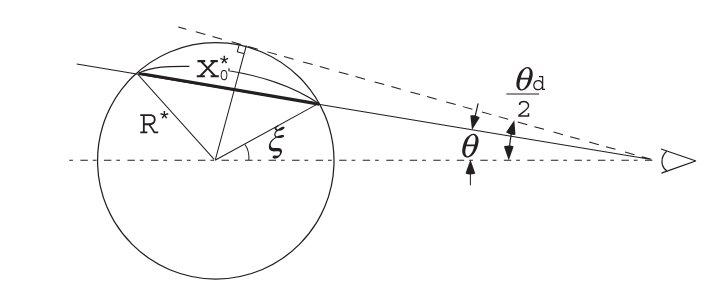
\includegraphics[width=0.5\textwidth]{C:/Users/henri/OneDrive/Documents/NTNU/Semester 10/Masteroppgave/Plots/Radiative_Transfer.png}
    \caption{Schematic view of the radiative transfer in a spherical ball of plasma. Image taken from \cite{Hirotani_2005}}
    \label{fig:Radiative_transfer}
\end{figure}
\subsection{Time-scales analysis}

